% Stage 2 results. Numbers come from results/final/stage2/paired.json (figgie.experiments.paired).

In each game, one seat is Jev and the other three seats are a fundamentalist, a bottom-feeder and a noise trader.
The twin arm plays the same games with the rule-based twin in Jev's seat. We compare the two arms game by game.
Each condition has \STAGETWOGAMES{} paired games (section~\ref{sec:limits} explains why not 40).
Figure~\ref{fig:paired} and Table~\ref{tab:s2} give the result for each condition.

\begin{figure}[t]
\centering
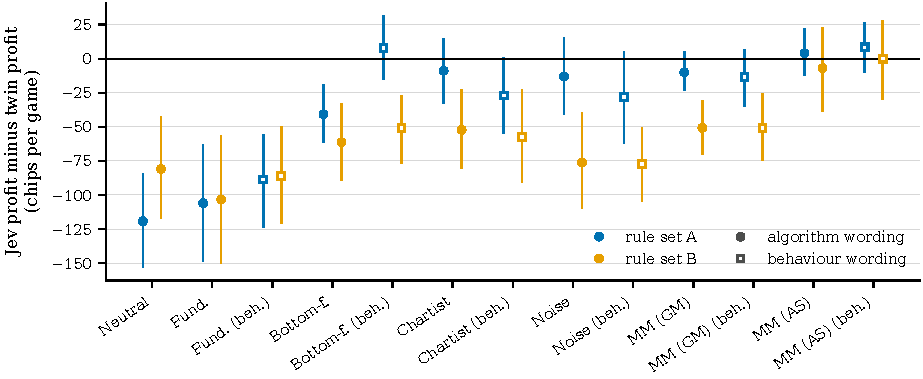
\includegraphics[width=\linewidth]{figures/stage2_paired.pdf}
\caption{Stage 2: mean profit difference, Jev minus its twin, in the same seat and the same games
(\STAGETWOGAMES{} games per point; 95\% cluster-bootstrap intervals). Below 0: Jev earns less than the rule-based
trader it plays. The twin of ``Neutral'' (no persona) is the fundamentalist.}
\label{fig:paired}
\end{figure}

\begin{table}[t]
\centering\small
\begin{tabular}{lrrlrrl}
\toprule
 & \multicolumn{3}{c}{Rule set A (order book)} & \multicolumn{3}{c}{Rule set B (open outcry)} \\
\cmidrule(lr){2-4}\cmidrule(lr){5-7}
Condition & Jev & Twin & Jev $-$ twin [95\%] & Jev & Twin & Jev $-$ twin [95\%] \\
\midrule
\inputtab{tables/stage2.tex}
\bottomrule
\end{tabular}
\caption{Stage 2: mean profit per game in the tested seat (chips), \STAGETWOGAMES{} paired games per cell.
$^*$: the 95\% interval does not include 0.}
\label{tab:s2}
\end{table}

\paragraph{Profit (RQ4, primary result).}
\begin{itemize}
\item \textbf{Jev earns less than its twin.} Over all 13 conditions of a rule set, the mean difference is
$-34$ chips per game in A (95\% interval [$-44$, $-25$]) and $-58$ in B ([$-68$, $-47$]).
\item \textbf{No condition is clearly better than its twin.} The difference is clearly below 0 in 5 of 13 conditions in
A and in 11 of 13 in B. Eight conditions in A are not clearly different from their twins: the bottom-feeder with the
behaviour wording, the chartist with the algorithm wording, both noise traders and all four market makers. In B, only
the two AS market-maker conditions are not clearly different.
\item \textbf{The largest losses are in the fundamentalist seat.} Jev with the fundamentalist persona loses 84 to 105
chips per game against the fundamentalist, in both rule sets and with both wordings. The fundamentalist is the only type
that earns money here (28 chips in A, 14 in B), so it is the hardest twin to equal.
\item \textbf{Close to the twin is not the same as good.} The market-maker twins earn little and Jev as a market maker
loses little. A small difference in these cells shows that both traders do little, not that Jev copies the twin
(their decisions overlap only 0.04--0.10 in stage~1).
\end{itemize}

\paragraph{Jev without a persona (H4a).} The neutral Jev earns less than the fundamentalist in the same seat and games
($-121$ chips in A, [$-158$, $-85$]; $-75$ in B, [$-111$, $-36$]). It also earns less than the noise trader in A
($-62$, [$-92$, $-31$]); in B, the difference to the noise trader is not clear ($-27$, [$-62$, 11]). So H4a holds only
in its first part: Jev with no persona is not better than a trader that decides at random.

\paragraph{Market rules (H2c) and wording.} Jev is closer to its twin in A than in B: the difference A $-$ B is
$+24$ chips per game ([11, 36]). So H2c is supported. The wording does not change profit: behaviour minus
algorithm is $+5$ chips ([$-6$, 16]). The regression gives the same result (Table~\ref{tab:reg}): the rule-set effect
is $+18$ ([3, 31]); the wording effect ($-2$) and its interaction with the rule set ($+13$) have intervals that
include 0.

\begin{table}[t]
\centering\small
\begin{tabular}{lrl}
\toprule
Term (reference: neutral Jev, rule set B, algorithm wording) & Estimate & 95\% interval \\
\midrule
Intercept & $-107$ & [$-134$, $-80$] \\
Rule set A & $+18$ & [3, 31] \\
Behaviour wording & $-2$ & [$-18$, 13] \\
Rule set A $\times$ behaviour wording & $+13$ & [$-7$, 32] \\
Type: fundamentalist & $0$ & [$-29$, 29] \\
Type: noise trader & $+43$ & [9, 76] \\
Type: chartist & $+58$ & [27, 88] \\
Type: bottom-feeder & $+62$ & [35, 86] \\
Type: market maker (GM) & $+66$ & [40, 90] \\
Type: market maker (AS) & $+95$ & [58, 127] \\
\midrule
Goal cards in the starting hand (second model) & $-7.1$ & [$-13.8$, $-0.8$] \\
\bottomrule
\end{tabular}
\caption{Regression of the paired difference $d_g$ on the design (988 pairs; cluster bootstrap over games, 1,000
resamples). With the goal-card covariate, all other estimates stay the same, because every condition plays the same
deals: the covariate is not correlated with the design.}
\label{tab:reg}
\end{table}

\paragraph{The starting hand.} Each extra goal card in the starting hand lowers the difference by 7 chips
([$-13.8$, $-0.8$]). A good hand helps the twin more than it helps Jev. This agrees with the belief result below: the
twin uses its cards to find the goal suit, and Jev does this badly.

\paragraph{Decisions and similarity (H4b).} Stage~1 measured, for each of the 24 persona cells, how similar Jev's
decisions are to the twin's (overlap). If similar decisions give similar profit, cells with a higher overlap should
have a smaller profit gap $|d|$. The result is the opposite: the rank correlation between overlap and $|d|$ is
$+0.52$ (permutation $p = 0.010$, 24 cells). The market makers cause most of this: they have the lowest overlap and a
small $|d|$ (see above). Inside one rule set the correlation is also positive but not clear (A: $+0.55$, $p = 0.07$;
B: $+0.27$, $p = 0.41$). So H4b is not supported. At the overlap levels that Jev reaches (at most 0.57), the profit gap
depends on the twin's type, not on how well Jev copies it.

\paragraph{How Jev trades (secondary; Table~\ref{tab:s2sec} in the appendix).}
\begin{itemize}
\item \textbf{Jev trades about twice as often as its twin}: 26 vs 12 trades per game in its seat in A, and 19 vs 9 in
B. The whole market trades more when Jev is in it (41 vs 30 trades per game in A, 26 vs 18 in B).
\item \textbf{Prices move further from the true value when Jev plays.} The mean distance between the trade price and
the true card value (10 for a goal card, 0 for other cards) is 7.3 with Jev and 5.9 with the twin in A, and 9.5 vs
6.1 in B.
\item \textbf{In B, the market rejects the twin's orders, not Jev's.} The twin has 17 rejected orders per game in B,
because its orders do not beat the best bid or ask. Jev has less than 1: its menu lists only prices that the rules
accept, and the few rejections come from quotes that change during the 0.3-second delay.
\end{itemize}

\paragraph{Belief in full games.} Jev's goal-suit belief in games is as poor as in stage~1: the mean log loss over all
decisions is 1.55 in A and 1.63 in B, against 1.27 and 1.28 for card counting at the same moments and 1.386 for a
uniform guess. Figure~\ref{fig:belief} shows that Jev's belief does not improve during the game, while the game
reveals more information with every trade. H1c is not supported in full games either.

\begin{figure}[t]
\centering
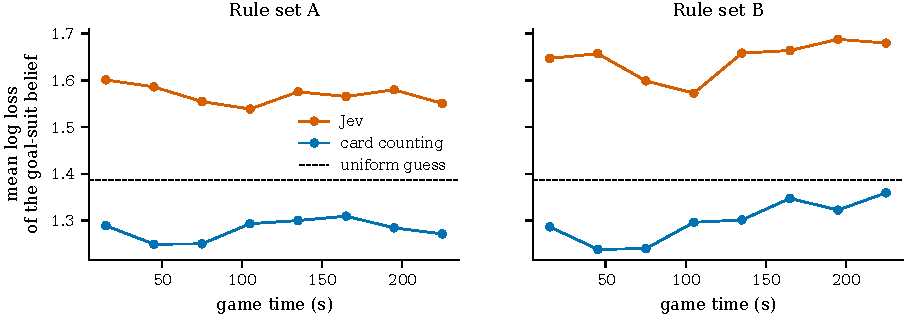
\includegraphics[width=\linewidth]{figures/stage2_belief_time.pdf}
\caption{Log loss of the goal-suit belief over game time (30-second bins), all Jev decisions in all conditions of a
rule set. Card counting is computed at the same moments from the same public information and Jev's own hand. Lower is
better; the dashed line is a uniform guess.}
\label{fig:belief}
\end{figure}
